\chapter{Quadro Terminal para Painel Led 10x4}
Este capítulo mostra os valores efetivos para a confecção do quadro para o Painel LED Full Color. Foram usados os métodos de dimensionamento explicados no Capítulo \ref{cap:calculos}. Nas próximas seções, serão apresentados os parâmetros de projeto utilizados, a tabela de carga, os diagramas unifilar e multifilar e uma representação gráfica do quadro (esquema funcional) nas opções simples. Ao final, há uma lista de materiais para montagem.

\section{Parâmetros de projeto}

O Painel Full Color Led 10x4 é composto por 40 gabinetes e deve ser alimentado com 14 cabos de força. Há três opções de resolução (P10, P8 e P5), cada uma com sua potência. A Tabela \ref{tab:pot_10x4} apresenta as informações de potência de cada gabinete, a quantidade de cabos ou grupos de até 3 gabinetes para conectar à rede elétrica e a quantidade de gabinetes e a potência total do Painel.

\begin{table}[htbp]
\caption{Potência Painel LED 10x4}
\centering
\begin{tabular}{cccccc}
\toprule
\multirow{2}{*}{Item} & \multirow{2}{*}{Tipo} & \multirow{2}{*}{Potência (W)} & \multicolumn{3}{c}{Painéis} \\
\cmidrule{4-6}
& & & Cabos  & Gabinete & Potência Total (W) \\
\midrule


37 & P8 & 630 & 14 & 40 & 25200 \\
38 & P5 & 684 & 14 & 40 & 27360 \\
39 & P10 & 540 & 14 & 40 & 21600 \\


\bottomrule
\end{tabular}
\label{tab:pot_10x4}
\end{table}

\section{Tabela de Carga}
%Para determinar a corrente de projeto, o disjuntor, a 
%Para determinar as cargas da Tabela \ref{tab:cargaT_10x4P10}, 
%a tensão de alimentação é de 220/380 V, o fatores de potência para cada circuito e geral foram 1 e 0,92 respectivamente. 
%
%
%\begin{table}[htbp]
%\centering
%\caption{Tabela de Carga QDT 10X4}
%\begin{tabular}{@{}llccccccccc@{}}
%
%\toprule
%Circuito &  &TUE &  L &  Cabo & DJ & \multicolumn{3}{c}{Fase} \\
%        & & Qtd &  (m) &  (mm²) & (A) & \\
%\midrule
%Grupo 1 & & 3 &  5 &  2,5 & 16 &  \\
%Grupo 2 & & 3 &  5 &  2,5 & 16 &  \\
%Grupo 3 & & 3 &  5 &  2,5 & 16 & \\
%Grupo 4 & &3 &  5 &  2,5 & 16 &    \\
%Grupo 5 && 3 &  5 &  2,5 & 16 &   \\
%Grupo 6 & & 3 & 5 &  2,5 & 16 &  \\
%Grupo 7 & &  3 & 5 & 2,5 & 16 &   \\
%Grupo 8 & & 3 &  5 & 2,5 & 16 &   \\
%Grupo 9 & & 3 &  5 & 2,5 & 16 &  \\
%Grupo 10 & &3 &  5 & 2,5 & 16 &    \\
%Grupo 11 & &3 &  5 & 2,5 & 16 &    \\
%Grupo 12 & &3 &  5 & 2,5 & 16 &  \\
%Grupo 13 & &2 &  5 & 2,5 & 16 &    \\
%Grupo 14 & &2 &  5 & 2,5 & 16 &    \\
%Comunicação & & 2 & 0,4 & 2,5 & 16 &  \\
%\bottomrule
%\end{tabular}
%\label{tab:cargaT_10x4P10}
%\end{table}

Neste quadro terão 14 circuitos para cada grupo de até 3 gabinetes e 1 circuito para tomadas internas utilizados na comunicação. A coluna TUE  indica a quantidade de gabinetes por grupo. Nas próximas colunas P é a potência dos equipamentos em Watts, L é o comprimento do cabo em m. Nas próximas colunas são os valores calculados para a corrente de projeto Ib, enquanto DT indica a corrente nominal do disjuntor, ambos em Ampere . Enquanto que as três últimas colunas indica a carga em  W para as fase R, fase S e Fase T.

\begin{table}[htbp]
\centering
\caption{Tabela de Carga QDT 200/380 V 10X4 T P10}

\begin{tabular}{@{}llccccccccc@{}}
%\begin{tabular}{llccccccccc}
\toprule
Circuito &  &TUE 540 & P & L & Ib & Cabo & DJ & \multicolumn{3}{c}{Fase} \\
        & & (W) & (W) & (m) & (A) & (mm²) & (A) & R & S & T \\
\midrule
Grupo 1 & & 3 & 1620 & 5 & 7,36 & 2,5 & 16 & 1620 &  &  \\
Grupo 2 & & 3 & 1620 & 5 & 7,36 & 2,5 & 16 &   & 1620 &  \\
Grupo 3 & & 3 & 1620 & 5 & 7,36 & 2,5 & 16 &   &   & 1620 \\
Grupo 4 & &3 & 1620 & 5 & 7,36 & 2,5 & 16 & 1620 &   &   \\
Grupo 5 && 3 & 1620 & 5 & 7,36 & 2,5 & 16 &   & 1620 &   \\
Grupo 6 & & 3 & 1620 & 5 & 7,36 & 2,5 & 16 &  &  & 1620 \\
Grupo 7 & &  3 & 1620 & 5 & 7,36 & 2,5 & 16 & 1620 &   &   \\
Grupo 8 & & 3 & 1620 & 5 & 7,36 & 2,5 & 16 &   & 1620 &   \\
Grupo 9 & & 3 & 1620 & 5 & 7,36 & 2,5 & 16 &   &   & 1620 \\
Grupo 10 & &3 & 1620 & 5 & 7,36 & 2,5 & 16 & 1620 &   &   \\
Grupo 11 & &3 & 1620 & 5 & 7,36 & 2,5 & 16 &   & 1620 &   \\
Grupo 12 & &3 & 1620 & 5 & 7,36 & 2,5 & 16 &   &   & 1620 \\
Grupo 13 & &2 & 1080 & 5 & 4,91 & 2,5 & 16 & 1080 &   &   \\
Grupo 14 & &2 & 1080 & 5 & 4,91 & 2,5 & 16 &   & 1080 &   \\
Comunicação & & 1 & 540 & 0,3 & 2,45 & 2,5 & 16 &  &  & 540 \\
Geral & & & 22140 & 80 & 36,61 & 10 & 10 & 7560 & 7560 & 7020 \\
\bottomrule
\end{tabular}
\label{tab:cargaT_10x4P10}
\end{table}


\subsection{Considerações}
As distribuição de paineis por grupo é uma sugestão visando uma melhor distribuição de carga nas fases.
Os tamanhos de fios de alimentação conforme parametros acima relacionados, aplicar correções quando o local de instalação tiver condições diferentes da aqui especificada.

\section{Diagrama Unifilar}

\subsection{Trifásico 127/220 V}

\subsection{Trifásico 127/220 V}

\section{Diagrama Multifilar}

\subsection{Trifásico 127/220 V}

\subsection{Trifásico 127/220 V}

\section{Representação geral de disposição dos componentes no quadro terminal}

\section{Lista de materiais}


\subsection{Trifásico 127/220 V}

\subsection{Trifásico 127/220 V}

\section{Montagem do Quadro}

\subsection{Identificações e adesivos}
\begin{enumerate}
\item Identificar as fase com anilhas. Os fios de neutro serão identificados pela cor azul clara, e o aterramento por cabos de cor verde ou verde e amarelo padrão aterramento. Nos caso não possíveis a distinção por cores usar anilhas de identificação.
\item Colocar adesivos de identificação de entrada de energia e saída para o painel dos fios de fase, aterramento e neutro.
\item  Colocar adesivo de identificação do lado externo da porta, da porta.
\item Advertência no quadro como Figura \ref{fig:advQD}
\end{enumerate}


\begin{figure}[htbp]
    \centering
    %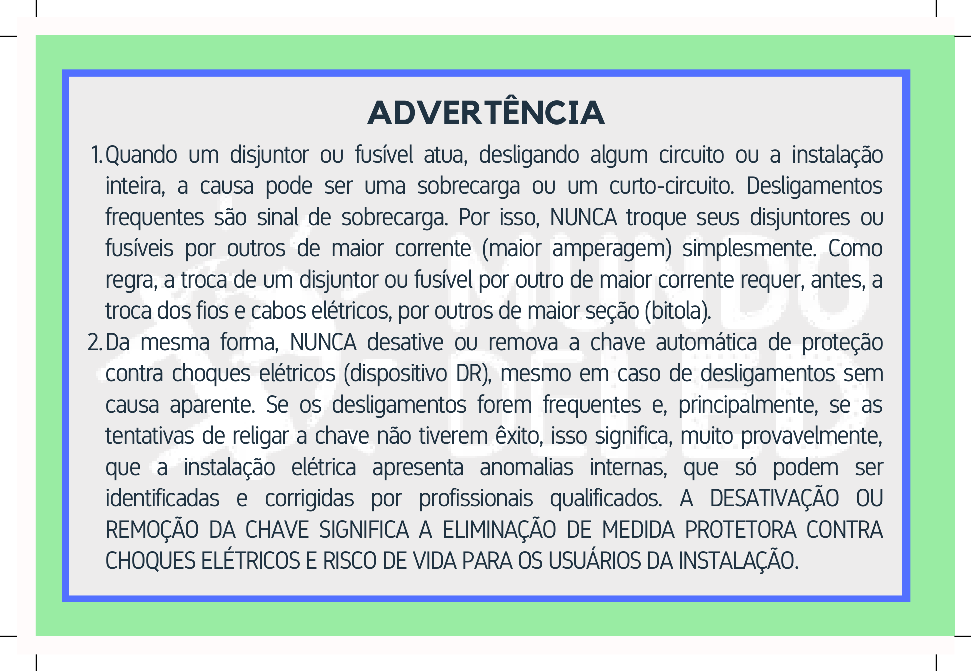
\includegraphics{image/EtiqAdvQD.pdf}
    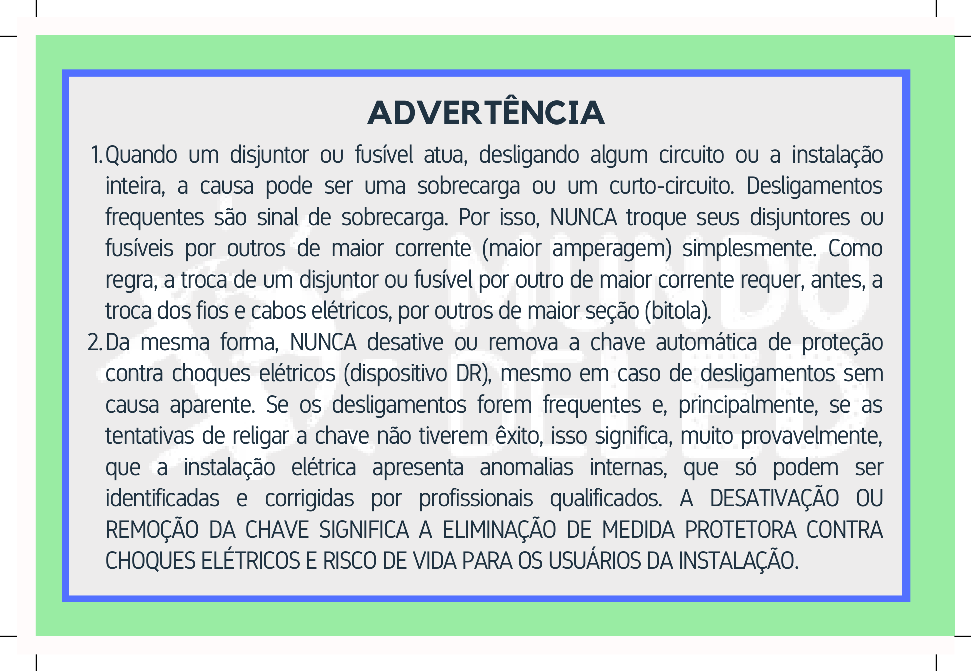
\includegraphics[scale=0.5]{image/EtiqAdvQD.pdf}
    \caption{Placa/ Adesivo de advertência para ser fixada no QD.}
    \label{fig:advQD}
\end{figure}